\documentclass[a4paper,10pt]{article}
\usepackage[utf8]{inputenc}
\usepackage[spanish]{babel}
\usepackage[affil-it]{authblk}
\usepackage{enumerate}
\usepackage{graphicx}
\usepackage{hyperref}
\usepackage{amsmath}
\usepackage{amssymb}
\usepackage{cancel}
\usepackage[usenames, dvipsnames]{color}
\usepackage{tikz}
\usepackage[labelfont=bf]{caption}
\usepackage{subcaption} %Multiple images
\usepackage{multicol} % Multiple columns
\usepackage{float}
\usepackage{cleveref}
 \usepackage{relsize} %bigger math symbols
\usepackage[margin=1.4in]{geometry}
\usepackage[titletoc,toc,title]{appendix}
\usepackage{enumitem}
\usetikzlibrary{calc}
\numberwithin{equation}{section}

%Appendices in spanish
\renewcommand{\appendixname}{Ap\'endices}
\renewcommand{\appendixtocname}{Ap\'endices}
\renewcommand{\appendixpagename}{Ap\'endices}

%Zero delimiter
\newcommand{\zerodel}{.\kern-\nulldelimiterspace}

%Columns separation
\setlength{\columnsep}{1cm}

%Indentation
\setlength{\parindent}{0ex}

%Multiple References

\crefrangelabelformat{equation}{(#3#1#4--#5\crefstripprefix{#1}{#2}#6)}

\usepackage{xparse}
\ExplSyntaxOn
\NewDocumentCommand{\mref}{m}{\quinn_mref:n {#1}}
\seq_new:N \l_quinn_mref_seq
\cs_new:Npn \quinn_mref:n #1
 {
  \seq_set_split:Nnn \l_quinn_mref_seq { , } { #1 }
  \seq_pop_right:NN \l_quinn_mref_seq \l_tmpa_tl
  ( % print the left parenthesis
  \seq_map_inline:Nn \l_quinn_mref_seq
    { \ref{##1},\nobreakspace } % print the first references
  \exp_args:NV \ref \l_tmpa_tl % print the last or only one
  ) % print the right parenthesis
 }
\ExplSyntaxOff


%Boxes

\newcommand*{\boxcolor}{blue}
\makeatletter
\renewcommand{\boxed}[1]{\textcolor{\boxcolor}{%
\tikz[baseline={([yshift=-1ex]current bounding box.center)}] \node [rectangle, minimum width=1ex,rounded corners,draw] {\normalcolor\m@th$\displaystyle#1$};}}
 \makeatother

%Constantes
\newcommand{\euler}{\mathrm{e}}
\newcommand{\im}{i}

%Lemas, teoremas, definiciones y pruebas
\newcommand{\definicion}{\textbf{Definición: }}
\newcommand{\lema}{\textbf{Lema: }}
\newcommand{\teorema}{\textbf{Teorema: }}
\newcommand{\prueba}{\textbf{Prueba: }}
\newcommand{\proposicion}{\textbf{Proposición: }}
\newcommand{\corolario}{\textbf{Corolario: }}


%opening
\title{Mecánica Clásica Tarea \# 9}
\author{Favio Vázquez\thanks{Correo: favio.vazquezp@gmail.com}}\affil{Instituto de Ciencias Nucleares. Universidad Nacional Autónoma de México.}
\date{}

\begin{document}

\makeatletter
\def\@maketitle{%
  \newpage
  \null
  \vskip 2em%
  \begin{center}%
  \let \footnote \thanks
    {\Large\bfseries \@title \par}%
    \vskip 1.5em%
    {\normalsize
      \lineskip .5em%
      \begin{tabular}[t]{c}%
        \@author
      \end{tabular}\par}%
    \vskip 1em%
    {\normalsize \@date}%
  \end{center}%
  \par
  \vskip 1.5em}
\makeatother

\maketitle

\section{Problema 1}

Tres masas iguales están acopladas por resortes iguales en las siguientes configuraciones:

$$
M - - k - - M - - k - - M
$$

$$
] - - k - - M - - k - - M - - k - - M
$$

$$ 
] - - k - - M - - k - - M - - k - - M - - k - -[
$$

$$
(M = \text{masa}\quad - - k - - = \text{resorte} \quad ][ = \text{pared})
$$

Para cada una de ellas encuentre los modos y las frecuencias normales de oscilación.

\vspace{.3cm}

\underline{Solución:} \vspace{.3cm}

Comenzaremos con una breve descripción del proceso que utilizaremos para resolver 
cada uno de los casos. Recordemos que en una vecindad suficientemente pequeña del 
punto de equilibrio, podemos aproximar al potencial como una forma bilineal simétrica 


\begin{equation}
 V = \frac{1}{2}\sum_{i,j=0}^n V_{ij}q^iq^j,
 \label{eq:energpoten1}
\end{equation}

donde 

\begin{equation}
 V_{ij} = \left\zerodel\frac{\partial^2 V}{\partial q^i \partial q^j}\right|_0,
 \label{eq:poten1}
\end{equation}

y que las condiciones para un mínimo nos indican que esta forma bilineal será 
positiva definida.

\vspace{.3cm}

Por otra parte, debido a que las velocidades generalizadas deben ser y permanecer 
pequeñas y a que las coordenadas permanecerán en una vecindad del origen, podemos 
aproximar la energía cinética, que también quedará a segundo orden, como 

\begin{equation}
 T = \frac{1}{2}\sum_{i,j=0}^n T_{ij}\dot{q}^i\dot{q}^j,
\end{equation}

donde $T_{ij}$ es la aproximación del tensor de inercia por sus valores en el origen.

\vspace{.3cm}

En un sentido muy resumido, necesitamos primero hallar una expresión para la energía 
cinética y la potencial en unas buenas coordenadas que tomen en cuenta la simetría 
del problema, luego debemos diagonalizar simultáneamente las dos matrices $T_{ij}$ 
y $V_{ij}$, aunque comúnmente si escogemos unas buenas coordenadas la matriz $T_{ij}$
ya estará en forma diagonal, dejándonos solo la diagonalización de la matriz $V_{ij}$
lo cual lo haremos utilizando el hecho de que $\det{(V_{ij}-\omega^2T_{ij})} = 0$, donde 
las $\omega$ son las frecuencias normales, lo cual nos permitirá obtener las mismas, 
y luego los modos normales. Esta metodología que utilizaremos no es exactamente la 
que vimos en clase, aunque es muy parecida debido a que se llegan a los mismos 
resultado de una forma similar, pero tal vez un poco más simple, y fue tomada de \cite{marion}. Por último un comentario sobre notación: 
denotaremos por\footnote{Numerando de izquierda a derecha,
es decir, que la partícula más a la izquierda será $\phi_1$ y la última de la 
derecha será $\phi_n$, para un sistema de $n$ partículas.} $\phi_i$ el desplazamiento de cada 
partícula con respecto a su posición de equilibrio cuando el sistema está totalmente 
relajado, y serán nuestras coordenadas generalizadas. 

\vspace{.3cm}

\textbf{Caso 1}:

$$
M - - k - - M - - k - - M
$$

\vspace{.3cm}

Para este sistema la energía cinética estará expresada como 

\begin{equation}
 T = \frac{1}{2}m(\dot{\phi_1}^2 + \dot{\phi_2}^2 + \dot{\phi_3}^2),
\end{equation}

y la energía potencial como

\begin{equation}
 V = \frac{k}{2}(\phi_2 - \phi_1)^2 + \frac{k}{2}(\phi_3 - \phi_2)^2.
 \label{eq:energpoten2}
\end{equation}

Para encontrar la matriz del potencial $V_{ij}$ utilizamos la ecuación \mref{eq:poten1},
por lo que tenemos que obtener las segundas derivadas de \mref{eq:energpoten2}, comencemos 
con las primeras derivadas,

\begin{align*}
 \frac{\partial V}{\partial \phi_1} &= - k (\phi_2 - \phi_1), \\
 \frac{\partial V}{\partial \phi_2} &= k (\phi_2 - \phi_1) - k (\phi_3 - \phi_2), \\
 \frac{\partial V}{\partial \phi_3} &= k (\phi_3 - \phi_2),
\end{align*}

ahora podemos obtener las segundas derivadas que buscamos,

\begin{align*}
 \frac{\partial^2 V}{\partial \phi_1^2} &= k, \\
 \frac{\partial^2 V}{\partial \phi_2^2} &= 2k, \\
 \frac{\partial^2 V}{\partial \phi_3^2} &= k, \\
 \frac{\partial^2 V}{\partial \phi_1\phi_2} = \frac{\partial^2 V}{\partial \phi_2\phi_1}&= -k, \\
 \frac{\partial^2 V}{\partial \phi_1\phi_3} = \frac{\partial^2 V}{\partial \phi_3\phi_1}  &= 0, \\
 \frac{\partial^2 V}{\partial \phi_2\phi_3} =  \frac{\partial^2 V}{\partial \phi_3\phi_2} &= -k.
\end{align*}

Entonces podemos escribir las matrices de la energía potencial y la energía 
cinética como

\begin{equation}
 V = \begin{pmatrix}
      k & -k & 0 \\
      -k & 2k & -k \\
      0 & -k & k
     \end{pmatrix},
\end{equation}

\begin{equation}
 T = \begin{pmatrix}
      m & 0 & 0 \\
      0 & m & 0 \\
      0 & 0 & m
     \end{pmatrix}.
\end{equation}

Debido a que la matriz para la energía cinética ya está diagonalizada, solo nos queda 
diagonalizar $V$, lo cual lo hacemos resolviendo

\begin{equation}
 \left| \begin{matrix}
	    k - \omega^2 m & -k & 0 \\
	    -k & 2k - \omega^2 m & -k \\
	    0 & -k & k - \omega^2 m
     \end{matrix}\right| = 0,
\end{equation}

Esta ecuación se reduce a 

\begin{equation}
 - 3 k^{2} m w^{2} + 4 k m^{2} w^{4} - m^{3} w^{6} = 0,
\end{equation}

Y de esta ecuación podemos encontrar las frecuencias normales que son:

\begin{align}
 \omega_1 &= 0, \\
 \omega_2 &= \sqrt{\frac{k}{m}}, \\
 \omega_3 &= \sqrt{\frac{3k}{m}}.
\end{align}

Para encontrar los modos normales hacemos uso de la ecuación

\begin{equation}
 \sum_j (V_{jk} - \omega^2_r T_{jk})a_{jr} = 0,
\end{equation}

donde las $a_{jr}$ son las amplitudes reales de la oscilación. Tenemos entonces 
para $k = 1$ 

\begin{equation}
 (V_{11} - \omega_r^2 T_{11})a_{1r} + (V_{21} - \omega_r^2 T_{21})a_{2r} = 0,
\end{equation}

\begin{equation}
 (k - \omega_r^2m)a_{1r} - k a_{2r} = 0 
\end{equation}

Sustituyendo para cada valor de $r$ tenemos,

\begin{align}
 r &= 1: \quad (k - \cancelto{0}{\omega_1^2}m)a_{11} - k a_{21} = 0 \Rightarrow 
 ka_{11} = ka_{21} \Rightarrow a_{11} = a_{21}, \\
 r &= 2: \quad (k - \omega_2^2m)a_{12} - ka_{22} = 0 \Rightarrow 
 \cancelto{0}{(k - k)a_{12}} - k a_{22} = 0 \Rightarrow a_{22} = 0, \\
 r &= 3: \quad (k - \omega_3^2m)a_{13} - ka_{23} = 0 \Rightarrow  
 -2ka_{13} - ka_{23} = 0 \Rightarrow a_{13} = \frac{a_{23}}{2}.
\end{align}

Para $k=2$,

\begin{equation}
 (V_{12} - \omega_r^2 \cancelto{0}{T_{12}})a_{1r} + (V_{22} - \omega_r^2 T_{22})a_{2r} + 
 (V_{32} - \omega_r^2 \cancelto{0}{T_{32}})a_{3r}= 0,
\end{equation}

\begin{equation}
 -ka_{1r} + (2k - \omega_r^2m)a_{2r} - ka_{3r} = 0,
\end{equation}

Sustituyendo para cada valor de $r$ tenemos,

\begin{align}
 r &=1: \quad -ka_{11} + (2k - \cancelto{0}{\omega_1^2}m)a_{21} - ka_{31} = 0 \Rightarrow
 ka_{11} - ka_{31} = 0 \Rightarrow a_{11} = a_{31}, \\
 r &=2: \quad -ka_{12} + (2k - \omega_2^2m)\cancelto{0}{a_{22}} - ka_{32} = 0 \Rightarrow
 -ka_{12} - ka_{32} = 0 \Rightarrow a_{12} = -a_{32},\\
 r &=3: \quad -ka_{13} + (2k - \omega_3^2m)a_{23} - ka_{33} = 0 \Rightarrow 
 -3ka_{13} - k_{33} = 0 \Rightarrow a_{33} = -3a_{13}.
\end{align}

Para $k=3$, 

\begin{equation}
 (\cancelto{0}{V_{13}} - \omega_r^2\cancelto{0}{T_{13}})a_{1r} +  (V_{23} - \omega_r^2\cancelto{0}{T_{23}})a_{2r} 
 +  (V_{33} - \omega_r^2T_{33})a_{3r} = 0,
\end{equation}

\begin{equation}
 -ka_{2r} + (k - \omega_r^2m)a_{3r} = 0,
\end{equation}

Sustituyendo para cada valor de $r$ tenemos,

\begin{align}
 r &= 1: \quad -ka_{21} + (k - \cancelto{0}{\omega_1^2}m)a_{31} = 0 \Rightarrow
 -ka_{21} + ka_{31} = 0 \Rightarrow a_{21} = a_{31}, \\
 r &= 2: \quad -k\cancelto{0}{a_{22}} + (k - \omega_2^2m)a_{32} = 0 \Rightarrow
 (k - k)a_{32} = 0 \Rightarrow a_{32} = - a_{12}, \\
 r &= 3: \quad -ka_{23} + (k - \omega_3^2m)a_{33} = 0 \Rightarrow
 -ka_{23} - 2ka_{33} = 0 \Rightarrow a_{33} = - \frac{a_{23}}{2}
\end{align}

Para hallar las coordenadas normales y los modos normales hacemos uso de las ecuaciones 
\cite{marion}

\begin{align}
 \phi_1 = a_{11}Q_1 + a_{12}Q_2 + a_{13}Q_3, \\
 \phi_2 = a_{21}Q_1 + a_{22}Q_2 + a_{23}Q_3, \\
 \phi_3 = a_{31}Q_1 + a_{32}Q_2 + a_{33}Q_3
\end{align}

Sustituyendo los valores para las $a_{jk}$, tenemos 

\begin{align}
 \phi_1 &= a_{11}Q_1 + a_{12}Q_2 + a_{13}Q_3, \\
 \phi_2 &= a_{11}Q_1 + 3a_{13}Q_3, \\
 \phi_3 &= a_{11}Q_1 - a_{12}Q_2 - 3a_{13}Q_3
\end{align}

Resolviendo para las coordenadas normales $Q_i$, 

\begin{align}
 Q_1 &= \frac{\phi_1 + \phi_3}{2a_{11}}\\
 Q_2 &= \frac{5\phi_1 + 5\phi_3 - 4\phi_2}{6a_{12}}\\
 Q_3 &= \frac{2\phi_2 - \phi_1 - \phi_3}{3a_{13}}
\end{align}

Los modos normales son 3 entonces, y ocurren cuando 

\begin{align}
 Q_1 &\Rightarrow \phi_1 + \phi_3 = 0 \Rightarrow \phi_1 = -\phi_3, \\
 Q_2 &\Rightarrow 5\phi_1 + 5\phi_3 - 4\phi_2 = 0 \Rightarrow \phi_2 = 
 - \frac{10}{4} \phi_1 = - \frac{10}{4} \phi_3, \\
 Q_3 &\Rightarrow 2\phi_2 - \phi_1 - \phi_3 = 0 \Rightarrow 
 \phi_1 = \phi_2 = \phi_3
\end{align}

\textbf{Caso 2}:

$$
] - - k - - M - - k - - M - - k - - M
$$

Para este sistema la energía cinética estará expresada como

\begin{equation}
 T = \frac{1}{2}m(\dot{\phi_1}^2 + \dot{\phi_2}^2 + \dot{\phi_3}^2),
\end{equation}

y la energía potencial como

\begin{equation}
 V = \frac{k}{2}\phi_1^2 + \frac{k}{2}(\phi_2 - \phi_1)^2 + \frac{k}{2}(\phi_3 - \phi_2)^2.
 \label{eq:energpoten3}
\end{equation}

Para encontrar la matriz del potencial $V_{ij}$ utilizamos la ecuación \mref{eq:poten1},
por lo que tenemos que obtener las segundas derivadas de \mref{eq:energpoten3}, comencemos 
con las primeras derivadas,

\begin{align*}
 \frac{\partial V}{\partial \phi_1} &= k\phi_1 - k (\phi_2 - \phi_1) = 2k\phi_1 - k\phi_2, \\
 \frac{\partial V}{\partial \phi_2} &= k (\phi_2 - \phi_1) - k (\phi_3 - \phi_2), \\
 \frac{\partial V}{\partial \phi_3} &= k (\phi_3 - \phi_2),
\end{align*}

ahora podemos obtener las segundas derivadas que buscamos,

\begin{align*}
 \frac{\partial^2 V}{\partial \phi_1^2} &= 2k, \\
 \frac{\partial^2 V}{\partial \phi_2^2} &= 2k, \\
 \frac{\partial^2 V}{\partial \phi_3^2} &= k, \\
 \frac{\partial^2 V}{\partial \phi_1\phi_2} = \frac{\partial^2 V}{\partial \phi_2\phi_1}&= -k, \\
 \frac{\partial^2 V}{\partial \phi_1\phi_3} = \frac{\partial^2 V}{\partial \phi_3\phi_1}  &= 0, \\
 \frac{\partial^2 V}{\partial \phi_2\phi_3} =  \frac{\partial^2 V}{\partial \phi_3\phi_2} &= -k.
\end{align*}

Entonces podemos escribir las matrices de la energía potencial y la energía 
cinética como

\begin{equation}
 V = \begin{pmatrix}
      2k & -k & 0 \\
      -k & 2k & -k \\
      0 & -k & k
     \end{pmatrix},
\end{equation}

\begin{equation}
 T = \begin{pmatrix}
      m & 0 & 0 \\
      0 & m & 0 \\
      0 & 0 & m
     \end{pmatrix}.
\end{equation}

Debido a que la matriz para la energía cinética ya está diagonalizada, solo nos queda 
diagonalizar $V$, lo cual lo hacemos resolviendo

\begin{equation}
 \left| \begin{matrix}
	    2k - \omega^2 m & -k & 0 \\
	    -k & 2k - \omega^2 m & -k \\
	    0 & -k & k - \omega^2 m
     \end{matrix}\right| = 0,
\end{equation}

Esta ecuación se reduce a 

\begin{equation}
 k^{3} - 6 k^{2} m w^{2} + 5 k m^{2} w^{4} - m^{3} w^{6} = 0,
 \label{eq:complex}
\end{equation}

Y de esta ecuación podemos encontrar las frecuencias normales que son:

\begin{align}
 \omega_1 &\approx \sqrt{\frac{k}{5m}}, \\
 \omega_2 &\approx \sqrt{\frac{3k}{2m}}, \\
 \omega_3 &\approx - \sqrt{\frac{7k}{2m}}.
\end{align}

Claramente estas frecuencias normales son aproximaciones debido a que la ecuación 
\mref{eq:complex} produce raíces complejas, pero con valores imaginarios despreciables, 
por lo tanto se aproximarán las primeras dos frecuencias a sus valores reales, 
y para simplificar los cálculos utilizaremos que $0.4450 \approx \sqrt{1/5}$, 
$1.2469 \approx \sqrt{3/2}$ y que $1.8019 \approx \sqrt{7/2}$.

\vspace{.3cm}

Para encontrar los modos normales hacemos uso de la ecuación

\begin{equation}
 \sum_j (V_{jk} - \omega^2_r T_{jk})a_{jr} = 0,
\end{equation}

donde las $a_{jr}$ son las amplitudes reales de la oscilación. Tenemos entonces 
para $k = 1$ 

\begin{equation}
 (V_{11} - \omega_r^2T_{11})a_{1r} + V_{21}a_{2r} + \cancelto{0}{V_{31}}a_{3r} = 0,
\end{equation}

\begin{equation}
 (2k - \omega_r^2m)a_{1r} - ka_{2r} = 0.
\end{equation}

Sustituyendo para cada valor de $r$ tenemos, 

\begin{align}
 r &= 1: (2k - \omega_1^2m)a_{11} - ka_{21} = 0 \Rightarrow a_{11} = \frac{5}{9}a_{12}, \\
 r &= 2: (2k - \omega_2^2m)a_{12} - ka_{22} = 0 \Rightarrow a_{12} = 2a_{22}, \\
 r &= 3: (2k - \omega_3^2m)a_{13} - ka_{23} = 0 \Rightarrow a_{13} = \frac{2}{11}a_{23}.
\end{align}

Para $k=2$

\begin{equation}
 V_{12}a_{1r} + (V_{22} - \omega_r^2T_{22})a_{2r} + V_{32}a_{3r} = 0
\end{equation}


\begin{equation}
 -ka_{1r} + (2k - \omega_r^2m)a_{2r} -k a_{3r} = 0
\end{equation}

Sustituyendo para cada valor de $r$ tenemos,

\begin{align}
 r &= 1: -ka_{11} + (2k - \omega_1^2m)a_{21} -k a_{31}  = 0 \Rightarrow 
 -a_{11} + \frac{9}{5}a_{21} = a_{31}, \\
 r &= 2: -ka_{12} + (2k - \omega_2^2m)a_{22} -k a_{32}  = 0 \Rightarrow 
 a_{32} = - \frac{3}{2}a_{22}, \\
 r &= 3: -ka_{13} + (2k - \omega_3^2m)a_{23} -k a_{33}  = 0 \Rightarrow 
 a_{33} \approx - \frac{2}{5} a_{23}.
\end{align}

Para $k=3$

\begin{equation}
 \cancelto{0}{V_{13}a_{1r}} + V_{23}a_{2r} + (V_{33} - \omega_r^2T_{33})a_{3r} = 0,
\end{equation}

\begin{equation}
 -ka_{2r} + (k - \omega_r^2m)a_{3r} = 0
\end{equation}

Sustituyendo para cada valor de $r$ tenemos,

\begin{align}
 r &= 1: -ka_{21} + (k - \omega_1^2m)a_{31} = 0 \Rightarrow  
 a_{21} =\frac{4}{5}a_{31},\\
 r &= 2: -ka_{22} + (k - \omega_2^2m)a_{32} = 0 \Rightarrow 
 a_{22} = -\frac{2}{3}a_{32}\\
 r &= 3: -ka_{23} + (k - \omega_3^2m)a_{33} = 0 \Rightarrow 
 a_{23} = - \frac{5}{2}a_{33}
\end{align}

Para hallar las coordenadas normales y los modos normales hacemos uso de las ecuaciones 

\begin{align}
 \phi_1 = a_{11}Q_1 + a_{12}Q_2 + a_{13}Q_3, \\
 \phi_2 = a_{21}Q_1 + a_{22}Q_2 + a_{23}Q_3, \\
 \phi_3 = a_{31}Q_1 + a_{32}Q_2 + a_{33}Q_3
\end{align}

Sustituyendo los valores para las $a_{jk}$, tenemos 

\begin{align}
 \phi_1 = a_{11}Q_1 + a_{12}Q_2 + a_{13}Q_3, \\
 \phi_2 = a_{21}Q_1 + \frac{1}{2}a_{12}Q_2 + a_{23}Q_3, \\
 \phi_3 = \frac{5}{4}a_{21}Q_1 + \frac{3}{4}a_{12}Q_2 - \frac{2}{5}a_{23}Q_3
\end{align}

Tenemos entonces las siguientes coordenadas normales,

\begin{align}
 Q_1 = \frac{(-3/2)\phi_2 + \phi_3 - (4a_{23}/5a_{13})((\phi_1/2)+\phi_2)}{(-1/4)a_{21} 
 - (6a_{11}a_{23}/5a_{13})}, \\
 Q_2 =  \frac{(3\phi_2/2)+\phi_3 - \frac{15}{4}a_{12}\left[ \frac{(-3/2)\phi_2 + \phi_3 - (4a_{23}/5a_{13})((\phi_1/2)+\phi_2)}{(-1/4)a_{21} 
 - (6a_{11}a_{23}/5a_{13})}\right]}{5a_{12}/4},\\
 Q_3 = \frac{(\phi_1/2)+\phi_2 - \frac{3}{2}a_{11}\left[\frac{(-3/2)\phi_2 + \phi_3 - (4a_{23}/5a_{13})((\phi_1/2)+\phi_2)}{(-1/4)a_{21} 
 - (6a_{11}a_{23}/5a_{13})} \right]}{5a_{13}}
\end{align}

Nos reservaremos el análisis de estos modos normales debido a la complejidad de 
las ecuaciones, que claramente se podrían reducir aún más, pero vemos que este caso 
tiene complicaciones, partiendo del hecho de que da soluciones complejas y tuvieron 
que hacerse muchas aproximaciones para llegar a estas coordenadas normales.

\vspace{.3cm}

\textbf{Caso 3}:

$$
] - - k - - M - - k - - M - - k - - M - - k - -[
$$

Para este sistema la energía cinética estará expresada como

\begin{equation}
 T = \frac{1}{2}m(\dot{\phi_1}^2 + \dot{\phi_2}^2 + \dot{\phi_3}^2),
\end{equation}

y la energía potencial como

\begin{equation}
 V = \frac{k}{2}\phi_1^2 + \frac{k}{2}(\phi_2 - \phi_1)^2 + \frac{k}{2}(\phi_3 - \phi_2)^2
 + \frac{k}{2}\phi_3^2.
 \label{eq:energpoten4}
\end{equation}

Para encontrar la matriz del potencial $V_{ij}$ utilizamos la ecuación \mref{eq:poten1},
por lo que tenemos que obtener las segundas derivadas de \mref{eq:energpoten4}, comencemos 
con las primeras derivadas,

\begin{align*}
 \frac{\partial V}{\partial \phi_1} &= k\phi_1 - k (\phi_2 - \phi_1) = 2k\phi_1 - k\phi_2, \\
 \frac{\partial V}{\partial \phi_2} &= k (\phi_2 - \phi_1) - k (\phi_3 - \phi_2), \\
 \frac{\partial V}{\partial \phi_3} &= k (\phi_3 - \phi_2) + k\phi_3 = 2k\phi_3 - k\phi_2,
\end{align*}

ahora podemos obtener las segundas derivadas que buscamos,

\begin{align*}
 \frac{\partial^2 V}{\partial \phi_1^2} &= 2k, \\
 \frac{\partial^2 V}{\partial \phi_2^2} &= 2k, \\
 \frac{\partial^2 V}{\partial \phi_3^2} &= 2k, \\
 \frac{\partial^2 V}{\partial \phi_1\phi_2} = \frac{\partial^2 V}{\partial \phi_2\phi_1}&= -k, \\
 \frac{\partial^2 V}{\partial \phi_1\phi_3} = \frac{\partial^2 V}{\partial \phi_3\phi_1}  &= 0, \\
 \frac{\partial^2 V}{\partial \phi_2\phi_3} =  \frac{\partial^2 V}{\partial \phi_3\phi_2} &= -k.
\end{align*}

Entonces podemos escribir las matrices de la energía potencial y la energía 
cinética como

\begin{equation}
 V = \begin{pmatrix}
      2k & -k & 0 \\
      -k & 2k & -k \\
      0 & -k & 2k
     \end{pmatrix},
\end{equation}

\begin{equation}
 T = \begin{pmatrix}
      m & 0 & 0 \\
      0 & m & 0 \\
      0 & 0 & m
     \end{pmatrix}.
\end{equation}

Debido a que la matriz para la energía cinética ya está diagonalizada, solo nos queda 
diagonalizar $V$, lo cual lo hacemos resolviendo

\begin{equation}
 \left| \begin{matrix}
	    2k - \omega^2 m & -k & 0 \\
	    -k & 2k - \omega^2 m & -k \\
	    0 & -k & 2k - \omega^2 m
     \end{matrix}\right| = 0,
\end{equation}

Esta ecuación se reduce a 

\begin{equation}
 4 k^{3} - 10 k^{2} m w^{2} + 6 k m^{2} w^{4} - m^{3} w^{6} = 0.
\end{equation}

Como hemos venido haciendo, de esta ecuación obtenemos las frecuencias normales que son:

\begin{align}
 \omega_1 &= \sqrt{\frac{2k}{m}} , \\
 \omega_2 &= \sqrt{\frac{(2+\sqrt{2})k}{m}}, \\
 \omega_3 &= \sqrt{\frac{(2-\sqrt{2})k}{m}}
\end{align}

Para encontrar los modos normales hacemos uso de la ecuación

\begin{equation}
 \sum_j (V_{jk} - \omega^2_r T_{jk})a_{jr} = 0,
\end{equation}

donde las $a_{jr}$ son las amplitudes reales de la oscilación. Debido a que ya debió
haber quedado claro el procedimiento para obtener las $a_{jr}$ solo escribiremos 
los resultados debajo

\begin{align}
 a_{21} = 0, \\
 a_{22} = -\sqrt{2}a_{12}, \\
 a_{23} = \sqrt{2}a_{13}, \\
 a_{11} = - a_{31}, \\
 a_{12} = a_{32}, \\
 a_{13} = a_{33}, \\
 a_{22} = -\sqrt{2}a_{32}, \\
 a_{23} = \sqrt{2}a_{33}
\end{align}

Para hallar las coordenadas normales y los modos normales hacemos uso de las ecuaciones 

\begin{align}
 \phi_1 = a_{11}Q_1 + a_{12}Q_2 + a_{13}Q_3, \\
 \phi_2 = a_{21}Q_1 + a_{22}Q_2 + a_{23}Q_3, \\
 \phi_3 = a_{31}Q_1 + a_{32}Q_2 + a_{33}Q_3
\end{align}

Sustituyendo los valores para las $a_{jk}$, tenemos 

\begin{align}
 \phi_1 = a_{11}Q_1 -\frac{1}{\sqrt{2}}a_{22} Q_2 + a_{13}Q_3, \\
 \phi_2 = a_{22}Q_2 + \sqrt{2}a_{33}Q_3, \\
 \phi_3 = - a_{11}Q_1 + -\frac{1}{\sqrt{2}}a_{22} Q_2 + a_{33}Q_3
\end{align}

Tenemos entonces las siguientes coordenadas normales,

\begin{align}
 Q_1 = \frac{\phi_1 - \phi_3}{2a_{11}}, \\
 Q_2 = \frac{-\phi_1 + \sqrt{2}\phi_2 - \phi_3}{2\sqrt{2}a_{22}}, \\
 Q_3 = \frac{\phi_1 + \sqrt{2}\phi_2 + \phi_3}{4a_{33}}.
\end{align}

Los modos normales son 3 entonces, y ocurren cuando 

\begin{align}
 Q_1 &\Rightarrow  \phi_1 = -\phi_3, \\
 Q_2 &\Rightarrow  \phi_2 = - \sqrt{2} \phi_1 = - \sqrt{2} \phi_3, \\
 Q_3 &\Rightarrow  \phi_1 = \sqrt{2}\phi_2 = \sqrt{2}\phi_3
\end{align}

\section{Problema 2}

Cuatro masas están acopladas cíclicamente por resortes iguales de constante $K$ con 
excepción de uno que tiene constante $k \ll K$. Encuentre a primer orden en $k$ los 
modos normales de oscilación. Hágalo para el caso en que las masas son distintas 
y para el caso en que son iguales. ¿Se podrá resolver este sistema de forma exacta?

\vspace{.3cm}

\underline{Solución:} \vspace{.3cm}

Podemos ver debajo una representación gráfica del sistema en cuestión,

\begin{figure}[H]
\center 
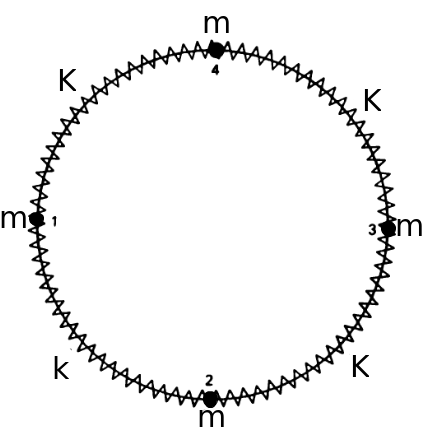
\includegraphics[scale=0.5]{problema2fig1}
 \caption{Cuatro masas acopladas cíclicamente.}
 \label{fig:problema2fig1}
\end{figure}

Comencemos estudiando el caso más general en el cual nas masas son distintas. 
Para estudiar el movimiento del sistema, denotaremos por $\phi_i$ el desplazamiento de cada 
partícula con respecto a su posición de equilibrio cuando el sistema está totalmente 
relajado, y serán nuestras coordenadas generalizadas.  por lo tanto la energía cinética 
del sistema será

\begin{equation}
 T = \frac{1}{2}m_1\phi_{1}^2 + \frac{1}{2}m_2\phi_{2}^2 + 
 \frac{1}{2}m_3\phi_{3}^2 + \frac{1}{2}m_4\phi_{4}^2,
\end{equation}

y la energía potencial

\begin{equation}
 V = \frac{1}{2}k(\phi_2 - \phi_1)^2 + \frac{1}{2}K(\phi_3 - \phi_2)^2
 + \frac{1}{2}K(\phi_4 - \phi_3)^2 + \frac{1}{2}K(\phi_1 - \phi_4)^2.
 \label{eq:energPotenCirc}
\end{equation}

La matriz para la energía cinética es entonces

\begin{equation}
 T = \begin{pmatrix}
      m_1 & 0 & 0 & 0 \\
      0 & m_2 & 0 & 0 \\
      0 & 0 & m_3 & 0 \\
      0 & 0 & 0 & m_4
     \end{pmatrix}
\end{equation}

Para encontrar la matriz del potencial $V_{ij}$ utilizamos la ecuación \mref{eq:poten1},
por lo que tenemos que obtener las segundas derivadas de \mref{eq:energPotenCirc}, comencemos 
con las primeras derivadas,

\begin{align*}
 \frac{\partial V}{\partial \phi_1} &= -k(\phi_2 - \phi_1) + K(\phi_1 - \phi_4) 
 = -k\phi_2 + k\phi_1 + K\phi_1 - K\phi_4 = \phi_1(K + k) -k\phi_2 - K\phi_4, \\
 \frac{\partial V}{\partial \phi_2} &= k(\phi_2 - \phi_1)  - K(\phi_3 - \phi_2)
 = k\phi_2 - k\phi_1 - K\phi_3 + K\phi_2 = \phi_2(K+k) - k\phi_1 - K\phi_3, \\
 \frac{\partial V}{\partial \phi_3} &= K(\phi_3 - \phi_2) - K(\phi_4 - \phi_3)
 = K\phi_3 - K\phi_2 - K\phi_4 + K\phi_3 = 2K\phi_3 - K\phi_2 - K\phi_4, \\
 \frac{\partial V}{\partial \phi_4} &=  K(\phi_4 - \phi_3) - K(\phi_1 - \phi_4)
 = K\phi_4 - K\phi_3 - K\phi_1 + K\phi_4 = 2K\phi_4 - K\phi_3 - K\phi_1 ,
\end{align*}

ahora podemos obtener las segundas derivadas que buscamos,

\begin{align*}
 \frac{\partial^2 V}{\partial \phi_1^2} &= K+k, \\
 \frac{\partial^2 V}{\partial \phi_2^2} &= K+k, \\
 \frac{\partial^2 V}{\partial \phi_3^2} &= 2K, \\
 \frac{\partial^2 V}{\partial \phi_4^2} &= 2K, \\
 \frac{\partial^2 V}{\partial \phi_1\phi_2} = \frac{\partial^2 V}{\partial \phi_2\phi_1}&= -k, \\
 \frac{\partial^2 V}{\partial \phi_1\phi_3} = \frac{\partial^2 V}{\partial \phi_3\phi_1}  &= 0, \\
 \frac{\partial^2 V}{\partial \phi_1\phi_4} =  \frac{\partial^2 V}{\partial \phi_4\phi_1} &= -K, \\
 \frac{\partial^2 V}{\partial \phi_2\phi_3} =  \frac{\partial^2 V}{\partial \phi_3\phi_2} &= -K, \\
 \frac{\partial^2 V}{\partial \phi_2\phi_4} =  \frac{\partial^2 V}{\partial \phi_4\phi_2} &= 0, \\ 
 \frac{\partial^2 V}{\partial \phi_3\phi_4} =  \frac{\partial^2 V}{\partial \phi_4\phi_3} &= -K.
\end{align*}

Podemos escribir entonces la matriz de la energía potencial como

\begin{equation}
 V = \begin{pmatrix}
      K+k & -k & 0 & -K \\
      -k & K+k & - K & 0 \\
      0 & - K & 2K & - K \\
      -K & 0 & - K & 2K
     \end{pmatrix}
\end{equation}

Debido a que la matriz para la energía cinética ya está diagonalizada, solo nos queda 
diagonalizar $V$, lo cual lo hacemos resolviendo

\begin{equation}
 \left|\begin{matrix}
      K+k - \omega^2m_1 & -k & 0 & -K \\
      -k & K+k - \omega^2m_2 & - K & 0 \\
      0 & - K & 2K -  \omega^2m_3 & - K \\
      -K & 0 & - K & 2K -  \omega^2m_4
     \end{matrix}\right| = 0.
\end{equation}

Esta ecuación se reduce a 

\begin{align}
 - K^{3} m_{1} w^{2} - K^{3} m_{2} w^{2} - K^{3} m_{3} w^{2} - K^{3} m_{4} w^{2} \\
 - 3 K^{2} k m_{1} w^{2} - 3 K^{2} k m_{2} w^{2} - 3 K^{2} k m_{3} w^{2} \\
 - 3 K^{2} k m_{4} w^{2} + 3 K^{2} m_{1} m_{2} w^{4} + 2 K^{2} m_{1} m_{3} w^{4}\\
 + K^{2} m_{1} m_{4} w^{4} + K^{2} m_{2} m_{3} w^{4} + 2 K^{2} m_{2} m_{4} w^{4} \\
 + K^{2} m_{3} m_{4} w^{4} + 2 K k m_{1} m_{3} w^{4} + 2 K k m_{1} m_{4} w^{4} \\
 + 2 K k m_{2} m_{3} w^{4} + 2 K k m_{2} m_{4} w^{4} + 2 K k m_{3} m_{4} w^{4} \\
 - 2 K m_{1} m_{2} m_{3} w^{6} - 2 K m_{1} m_{2} m_{4} w^{6} \\
 - K m_{1} m_{3} m_{4} w^{6} - K m_{2} m_{3} m_{4} w^{6} - k m_{1} m_{3} m_{4} w^{6} \\
 - k m_{2} m_{3} m_{4} w^{6} + m_{1} m_{2} m_{3} m_{4} w^{8} = 0
\end{align}

Vemos que resolver esta expresión analíticamente no es posible, ni 
los programas especializados podrían hacerlo, pero si se puede resolver numéricamente,
no haremos esto porque sale de la solución del problema. Lo que si podemos hacer 
es intentar resolver el sistema cuando las masas son iguales, en este caso

\begin{equation}
 \left|\begin{matrix}
      K+k - \omega^2m & -k & 0 & -K \\
      -k & K+k - \omega^2m & - K & 0 \\
      0 & - K & 2K -  \omega^2m & - K \\
      -K & 0 & - K & 2K -  \omega^2m
     \end{matrix}\right| = 0.
\end{equation}


Esta ecuación se reduce a 

\begin{equation}
 - 4 K^{3} m w^{2} - 12 K^{2} k m w^{2} + 10 K^{2} m^{2} w^{4} + 
 10 K k m^{2} w^{4} - 6 K m^{3} w^{6} - 2 k m^{3} w^{6} + m^{4} w^{8} = 0,
\end{equation}

y de esta ecuación podemos encontrar las frecuencias normales que son

\begin{align}
 \omega_1 &= 0, \\
 \omega_2 &= \sqrt{\frac{2K}{m}}, \\
 \omega_3 &= \sqrt{\frac{2K+k-\sqrt{2K+2Kk}}{m}} \approx 
 \sqrt{\frac{2K-\sqrt{2K}}{m}}, \\
 \omega_4 &=  \sqrt{\frac{2K+k+\sqrt{2K+2Kk}}{m}} \approx 
 \sqrt{\frac{2K+\sqrt{2K}}{m}},
\end{align}

recordando que debido a que $k\ll K$ entonces $K+k \approx K$ y $Kk \approx 0$.

\vspace{.3cm}

Para encontrar los modos normales hacemos uso de la ecuación

\begin{equation}
 \sum_j (V_{jk} - \omega^2_r T_{jk})a_{jr} = 0,
\end{equation}

donde las $a_{jr}$ son las amplitudes reales de la oscilación. Tenemos entonces 
para $k = 1$ 

\begin{equation}
 (V_{11} - \omega_r^2 T_{11})a_{1r} + (V_{21} - \omega_r^2 \cancelto{0}{T_{21}})a_{2r} 
 (\cancelto{0}{V_{31}} - \omega_r^2 \cancelto{0}{T_{31}})a_{3r} +
 (V_{41} - \omega_r^2 \cancelto{0}{T_{41}})a_{4r} = 0,
\end{equation}

\begin{equation}
 (K - \omega_r^2m)a_{1r} - ka_{2r} -Ka_{4r} = 0
\end{equation}

Sustituyendo para cada valor de $r$ tenemos,

\begin{align*}
 r &= 1: \quad  (K - \cancelto{0}{\omega_1^2}m_1)a_{11} - ka_{21} - Ka_{41}= 0 \Rightarrow
 a_{11}= \frac{ka_{21} + Ka_{41}}{K}, \\
 r &= 2: \quad (K - \omega_2^2m)a_{12} - ka_{22} - Ka_{42} = 0 \Rightarrow
 a_{12} = - \frac{ka_{22} + Ka_{42}}{K}, \\
 r &= 3: \quad (K - \omega_3^2m)a_{13} - ka_{23} - Ka_{43} = 0 \Rightarrow
 a_{13} = \frac{ka_{23} + Ka_{43}}{-K + \sqrt{2K}}, \\
 r &= 4: \quad (K - \omega_4^2m)a_{14} - ka_{24} - Ka_{44} = 0 \Rightarrow  
 a_{14} = \ \frac{ka_{24} + Ka_{44}}{-K - \sqrt{2K}}.
 \end{align*}
 
Para $k = 2$ 

\begin{equation}
 (V_{12} - \omega_r^2 \cancelto{0}{T_{12}})a_{1r} + (V_{22} - \omega_r^2 T_{22})a_{2r} 
  + (V_{32} - \omega_r^2 \cancelto{0}{T_{32}})a_{3r} + (\cancelto{0}{V_{42}} - \omega_r^2 \cancelto{0}{T_{42}})= 0,
\end{equation}

\begin{equation}
 -ka_{1r} + (K - \omega_r^2m)a_{2r} - Ka_{3r} = 0.
\end{equation}

Sustituyendo para cada valor de $r$ tenemos,

\begin{align}
 r &= 1: \quad -ka_{11} + (K - \cancelto{0}{\omega_1^2}m)a_{21} - Ka_{31} = 0 \Rightarrow 
 a_{21} = - \frac{ka_{11} + Ka_{31}}{K}, \\
 r &= 2: \quad -ka_{12} + (K - \omega_2^2m)a_{22} - Ka_{32} = 0 \Rightarrow
 a_{22} = - \frac{ka_{12} + Ka_{32}}{K}, \\
 r &= 3: \quad -ka_{13} + (K - \omega_3^2m)a_{23} - Ka_{33} = 0 \Rightarrow
 a_{33} = \frac{ka_{13} + (K - \sqrt{2K})a_{23}}{K}, \\
 r &= 4: -ka_{14} + (K - \omega_4^2m)a_{24} - Ka_{34} = 0 \Rightarrow 
 a_{34} = \frac{ka_{14} + (K + \sqrt{2K})a_{24}}{K},
\end{align}

Para $k = 3$ 

\begin{equation}
 (\cancelto{0}{V_{13}} - \omega_r^2 \cancelto{0}{T_{13}})a_{1r} + (V_{23} - \omega_r^2 \cancelto{0}{T_{23}})a_{2r} 
  + (V_{33} - \omega_r^2 T_{33})a_{3r} + (V_{43} - \omega_r^2 \cancelto{0}{T_{43}})a_{4r} = 0,
\end{equation}

\begin{equation}
 - Ka_{2r} + (2K - \omega_r^2m)a_{3r} - Ka_{4r} = 0.
\end{equation}

Sustituyendo para cada valor de $r$ tenemos,

\begin{align}
 r &= 1: \quad - Ka_{21} + (2K - \cancelto{0}{\omega_1^2}m)a_{31} - Ka_{41} = 0 \Rightarrow
 a_{41} = a_{21} + 2a_{31}, \\
 r &= 2: \quad - Ka_{22} + (2K - \omega_2^2m)a_{32} - Ka_{42} = 0 \Rightarrow
 a_{44} = a_{22}, \\
 r &= 3: \quad - Ka_{23} + (2K - \omega_3^2m)a_{33} - Ka_{43} = 0 \Rightarrow
 a_{23} = \frac{- Ka_{43} + \sqrt{2K}a_{33}}{K}, \\
 r &= 4: \quad - Ka_{24} + (2K - \omega_4^2m)a_{34} - Ka_{44} = 0 \Rightarrow
 a_{24} = \frac{- Ka_{44} - \sqrt{2K}a_{34}}{K}.
\end{align}

Para $k = 4$ 

\begin{equation}
 (V_{14} - \omega_r^2 \cancelto{0}{T_{14}})a_{1r} + (\cancelto{0}{V_{24}} - \omega_r^2 \cancelto{0}{T_{24}})a_{2r} 
  + (V_{34} - \omega_r^2 \cancelto{0}{T_{34}})a_{3r} + (V_{44} - \omega_r^2 T_{44})a_{4r} = 0,
\end{equation}

\begin{equation}
 - Ka_{1r} - Ka_{3r} + (2K - \omega_r^2m)a_{4r} = 0.
\end{equation}

Sustituyendo para cada valor de $r$ tenemos

\begin{align}
 r &= 1: \quad - Ka_{11} - Ka_{31} + (2K - \cancelto{0}{\omega_1^2}m)a_{41} = 0 \Rightarrow 
 a_{41} = \frac{a_{11} + a_{31}}{2}, \\
 r &= 2: \quad - Ka_{12} - Ka_{32} + (2K - \omega_2^2m)a_{42} = 0 \Rightarrow 
 a_{32} = - a_{12}, \\
 r &= 3: \quad - Ka_{13} - Ka_{33} + (2K - \omega_3^2m)a_{43} = 0 \Rightarrow 
 a_{33} = \frac{-Ka_{13} + \sqrt{2K}a_{43}}{K}, \\
 r &= 4: \quad - Ka_{14} - Ka_{34} + (2K - \omega_4^2m)a_{44} = 0 \Rightarrow 
 a_{44} = \frac{-K a_{34} + Ka_{14}}{\sqrt{2K}} .
\end{align}

Entonces las ecuaciones 

\begin{align}
 \phi_1 = a_{11}Q_1 + a_{12}Q_2 + a_{13}Q_3 + a_{14}Q_4, \\
 \phi_2 = a_{21}Q_1 + a_{22}Q_2 + a_{23}Q_3 + a_{24}Q_4, \\
 \phi_3 = a_{31}Q_1 + a_{32}Q_2 + a_{33}Q_3 + a_{34}Q_4, \\
 \phi_4 = a_{41}Q_1 + a_{42}Q_2 + a_{43}Q_3 + a_{44}Q_4,
\end{align}

pueden escribirse como

\begin{align*}
 \phi_1 &= a_{11}Q_1 + a_{12}Q_2 + a_{13}Q_3 + a_{14}Q_4, \\
 \phi_2 &= - \frac{ka_{11} + Ka_{31}}{K}Q_1 + \frac{-K a_{34} + Ka_{14}}{\sqrt{2K}}Q_2 + 
 \frac{- Ka_{43} + \sqrt{2K}a_{33}}{K}Q_3 + \frac{- Ka_{44} - \sqrt{2K}a_{34}}{K}Q_4, \\
 \phi_3 &= a_{31}Q_1 - a_{12}Q_2 + \frac{-Ka_{13} + \sqrt{2K}a_{43}}{K}Q_3 + 
 \frac{ka_{14} + (K + \sqrt{2K})a_{24}}{K}Q_4, \\
 \phi_4 &=  \frac{a_{11} + a_{31}}{2}Q_1 + a_{42}Q_2 + a_{43}Q_3 + 
 \frac{-K a_{34} + Ka_{14}}{\sqrt{2K}}Q_4,
\end{align*}

Esta ecuación es muy compleja y aún con la aproximación de que $K/K \approx 0$ no 
se pudo encontrar una expresión lo suficientemente simple para las coordenadas normales 
para poder hacer algún tipo de análisis del sistema. Pero con las ecuaciones que quedan 
planteadas para las coordenadas normales, y un software numérico se podría hacer este 
cálculo. No es extremadamente complicado el movimiento del sistema, y se pudo aproximar 
con \texttt{SymPy}\footnote{\href{http://www.sympy.org/en/index.html}{http://www.sympy.org/en/index.html}}. 
El resultado para los vectores propios y coordenadas normales se encuentran en el siguiente 
NoteBook de IPython, en la casilla ``\#Problema 3'', \href{https://github.com/FavioVazquez/MecanicaClasica-PCF/blob/master/Tarea9/Matrices.ipynb}{\color{blue}.::Link al Notebook::.}. 
Este análisis ya escapa de la tarea y se deja al lector interesado acceder al repositorio 
y ver el resultado numérico, también se puede encontrar información sobre este tipo 
de sistemas en \cite{kotkin}.


\section{Problema 3}

Encuentre las frecuencias normales de oscilación de un péndulo esférico doble: (una 
masa $m_1$ se mueve sobre una esfera de radio $R_1$ centrada en un punto fijo del 
espacio, otra masa $m_2$ se mueve sobre una esfera de radio $R_2$ centrada en la 
primera masa, todo ellos en presencia de la gravedad). Describa los modos normales 
de este sistema.

\vspace{.3cm}

\underline{Solución:} \vspace{.3cm}

En la figura de abajo se muestra una esquematización del péndulo doble esférico
con el que trabajaremos

\begin{figure}[H]
 \center 
 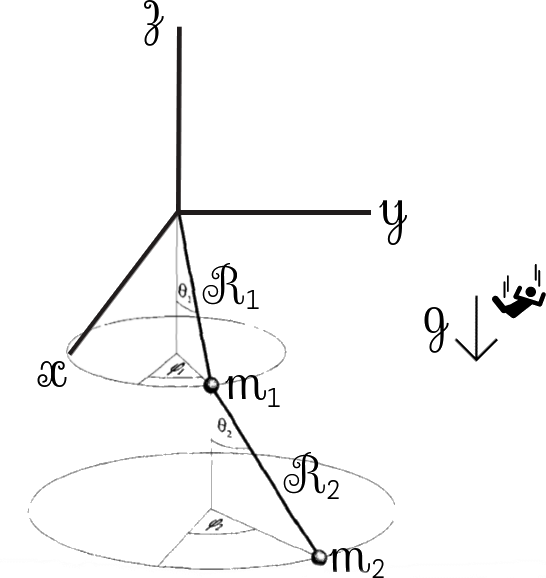
\includegraphics[scale=0.43]{problema3fig1}
 \caption{Péndulo doble esférico}
 \label{fig:problema3fig1}
\end{figure}

Hemos colocado el origen en el punto fijo del primer péndulo, la masa 1 tendrá 
coordenadas $(x,y,z)$, a la masa 2 le asignaremos las coordenadas 
$(u,v,w)$ para simplificar la notación. Aunque están en la imagen dibujados, 
no utilizaremos los ángulos como coordenadas generalizadas ya que complican 
el análisis del sistema. Tendemos entonces 6 coordenadas generalizadas para 
describir el sistema, pero existen dos constricciones holonómicas, que son 

\begin{align}
 x^2 + y^2 + z^2 = R_1^2, \\
 (x - u)^2 + (y-v)^2 + (z-w)^2 = R_2^2.
\end{align}

Por lo que entonces tenemos un sistema con 4 grados de libertad. Solo como una nota relevante, 
la variedad de configuración de este sistema es $\mathbb{S}^2 \times \mathbb{S}^2$, 
la cual es bastante difícil de describir en detalle.

\vspace{.3cm}

Siguiendo la típica receta, escribamos ahora una expresión para la energía cinética y 
la potencial,

\begin{equation}
 T = \frac{1}{2}m_1(\dot{x}^2+\dot{y}^2+\dot{z}^2) 
 + \frac{1}{2}m_2(\dot{u}^2+\dot{v}^2+\dot{w}^2),
\end{equation}

\begin{equation}
 V = - m_1gz - m_2gw.
\end{equation}

De las constricciones tenemos que 

\begin{align*}
 z &= \sqrt{R_1^2 - x^2 - y^2}, \\
 w &= z - \sqrt{R_2^2 - (x-u)^2 - (y-v)^2} = \sqrt{R_1^2 - x^2 - y^2} - 
 \sqrt{R_2^2 - (x-u)^2 - (y-v)^2}
\end{align*}

Por lo tanto $V$ queda expresada como 

\begin{equation}
 V = - m_1g\sqrt{R_1^2 - x^2 - y^2} - m_2g\sqrt{R_1^2 - x^2 - y^2} + 
 m_2 g  \sqrt{R_2^2 - (x-u)^2 - (y-v)^2}
 \label{eq:energPotenDoble}
\end{equation}

Como queremos estudiar el sistema bajo pequeñas oscilaciones, notamos que esto ocurre 
cuando se mantiene que $z \approx R_1$ y $w \approx R_1 + R_2$, por lo que $\dot{z} = 
\dot{w} = 0$, y la energía cinética es entonces 

\begin{equation}
 T = \frac{1}{2}m_1(\dot{x}^2+\dot{y}^2) 
 + \frac{1}{2}m_2(\dot{u}^2+\dot{v}^2),
\end{equation}

Para encontrar la matriz del potencial $V_{ij}$ utilizamos la ecuación \mref{eq:poten1},
por lo que tenemos que obtener las segundas derivadas de \mref{eq:energPotenDoble}, comencemos 
con las primeras derivadas,

\begin{align*}
 \frac{\partial V}{\partial x} &= - \frac{m_2 g (x-u)}{\sqrt{R_2^2-(u-x)^2-(v-y)^2}}+
 \frac{m_1 g x}{\sqrt{R_1^2-x^2-y^2}}+ \frac{m_2 g x}{\sqrt{R_1^2-x^2-y^2}} \\
 \frac{\partial V}{\partial y} &=  - \frac{g m_2 (y-v)}{\sqrt{R_2^2-(x-u)^2-(y-v)^2}} + 
 \frac{g m_1 y}{\sqrt{R_1^2-x^2-y^2}}+ \frac{g m_2 y}{\sqrt{R_1^2-x^2-y^2}} \\
 \frac{\partial V}{\partial u} &=  \frac{g m_2 (x-u)}{\sqrt{R_2^2-(x-u)^2-(y-v)^2}} \\
 \frac{\partial V}{\partial v} &=  \frac{g m_2 (y-v)}{\sqrt{R_2^2-(x-u)^2-(y-v)^2}},
\end{align*}

Utilizando las expresiones para las constricciones podemos transformar estas derivadas
en, recordando que $z \approx R_1$ y $w \approx R_1 + R_2$

\begin{align*}
 \frac{\partial V}{\partial x} &= \frac{m_2 g (x-u)}{w-z}+
 \frac{m_1 g x}{z}+ \frac{m_2 g x}{z} = \frac{gm_2(x-u)}{R_2} + \frac{xg (m_1+m_2)}{R_1}\\
 \frac{\partial V}{\partial y} &=  \frac{g m_2 (y-v)}{w-z} + 
 \frac{g m_1 y}{z}+ \frac{g m_2 y}{z}= \frac{gm_2(y-v)}{R_2} + \frac{yg (m_1+m_2)}{R_1} \\
 \frac{\partial V}{\partial u} &=  \frac{g m_2 (x-u)}{z-w} = 
 - \frac{g m_2 (x-u)}{R_2}\\
 \frac{\partial V}{\partial v} &=  \frac{g m_2 (y-v)}{z-w} = 
  -\frac{g m_2 (y-v)}{R_2},
\end{align*}

ahora podemos obtener las segundas derivadas que buscamos,

\begin{align*}
 \frac{\partial^2 V}{\partial x^2} &= \frac{gm_2}{R_2} + \frac{g(m_1 + m_2)}{R_1}, \\
 \frac{\partial^2 V}{\partial y^2} &= \frac{gm_2}{R_2} + \frac{g(m_1 + m_2)}{R_1}, \\
 \frac{\partial^2 V}{\partial u^2} &= \frac{gm_2}{R_2}, \\
 \frac{\partial^2 V}{\partial v^2} &= \frac{gm_2}{R_2}, \\
 \frac{\partial^2 V}{\partial x\partial y} = \frac{\partial^2 V}{\partial y \partial x}&= 0, \\
 \frac{\partial^2 V}{\partial x \partial u} = \frac{\partial^2 V}{\partial u \partial x}  &= - \frac{gm_2}{R_2}, \\
 \frac{\partial^2 V}{\partial x \partial v} =  \frac{\partial^2 V}{\partial v \partial x} &= 0, \\
 \frac{\partial^2 V}{\partial y \partial u} =  \frac{\partial^2 V}{\partial u \partial y} &= 0, \\
 \frac{\partial^2 V}{\partial y \partial v} =  \frac{\partial^2 V}{\partial v \partial y} &= -\frac{gm_2}{R_2} , \\ 
 \frac{\partial^2 V}{\partial u \partial v} =  \frac{\partial^2 V}{\partial v \partial u} &= 0.
\end{align*}

Podemos escribir entonces la matriz de la energía potencial como

\begin{equation}
 V = \begin{pmatrix}
      \frac{gm_2}{R_2} + \frac{g(m_1 + m_2)}{R_1} & 0 & - \frac{gm_2}{R_2} & 0 \\
      0 & \frac{gm_2}{R_2} + \frac{g(m_1 + m_2)}{R_1} & 0 & - \frac{gm_2}{R_2} \\
      - \frac{gm_2}{R_2} & 0 & \frac{gm_2}{R_2} & 0 \\
      0 & - \frac{gm_2}{R_2} & 0 & \frac{gm_2}{R_2}
     \end{pmatrix}
\end{equation}

y la matriz de la energía cinética como 

\begin{equation}
 T = \begin{pmatrix}
      m_1 & 0 & 0 & 0 \\
      0 & m_1 & 0 & 0 \\
      0 & 0 & m_2 & 0 \\
      0 & 0 & 0 & m_2
     \end{pmatrix}.
\end{equation}

Si nos mantenemos en el caso en que las longitudes de las barras que sostienen a las 
masas son diferentes, y también la magnitud de las mismas, entonces tendríamos que 
diagonalizar la matriz de la energía potencial para así encontrar las frecuencias 
normales y luego los modos normales, resolviendo lo siguiente 

\begin{equation}
 \left| \begin{matrix}
      \frac{gm_2}{R_2} + \frac{g(m_1 + m_2)}{R_1} - \omega^2m_1 & 0 & - \frac{gm_2}{R_2} & 0 \\
      0 & \frac{gm_2}{R_2} + \frac{g(m_1 + m_2)}{R_1} - \omega^2m_1 & 0 & - \frac{gm_2}{R_2} \\
      - \frac{gm_2}{R_2} & 0 & \frac{gm_2}{R_2} - \omega^2m_2 & 0 \\
      0 & - \frac{gm_2}{R_2} & 0 & \frac{gm_2}{R_2} - \omega^2m_2
        \end{matrix}\right| = 0,
\end{equation}

que se reduce a la siguiente expresión

\begin{align*}
 m_{1}^{2} m_{2}^{2} \omega^{8} - \frac{2 g}{R_{2}} m_{1}^{2} m_{2}^{2} \omega^{6} -
 \frac{2 g}{R_{2}} m_{1} m_{2}^{3} \omega^{6} + \frac{g^{2} m_{1}^{2}}{R_{2}^{2}} m_{2}^{2} \omega^{4} + \\
 \frac{2 m_{1}}{R_{2}^{2}} g^{2} m_{2}^{3} \omega^{4} + \frac{g^{2} m_{2}^{4}}{R_{2}^{2}} \omega^{4} - 
 \frac{2 g}{R_{1}} m_{1}^{2} m_{2}^{2} \omega^{6} - \frac{2 g}{R_{1}} m_{1} m_{2}^{3} \omega^{6} + 
 \frac{4 g^{2} m_{1}^{2} m_{2}^{2}}{R_{1} R_{2}} \omega^{4} + \\
 \frac{6 g^{2} m_{1} m_{2}^{3}}{R_{1} R_{2}} \omega^{4} + 
 \frac{2 g^{2} m_{2}^{4} \omega^{4}}{R_{1} R_{2}} - 
 \frac{2 g^{3} m_{1}^{2} m_{2}^{2}}{R_{1} R_{2}^{2}} \omega^{2} - 
 \frac{4 g^{3} m_{1} m_{2}^{3}}{R_{1} R_{2}^{2}} \omega^{2} - \\
 \frac{2 g^{3} m_{2}^{4} \omega^{2}}{R_{1} R_{2}^{2}} + 
 \frac{g^{2} m_{1}^{2}}{R_{1}^{2}} m_{2}^{2} \omega^{4} + 
 \frac{2 m_{1}}{R_{1}^{2}} g^{2} m_{2}^{3} \omega^{4} + 
 \frac{g^{2} m_{2}^{4}}{R_{1}^{2}} \omega^{4} - \\
 \frac{2 g^{3} m_{1}^{2} m_{2}^{2}}{R_{1}^{2} R_{2}} \omega^{2} - 
 \frac{4 g^{3} m_{1} m_{2}^{3}}{R_{1}^{2} R_{2}} \omega^{2} - 
 \frac{2 g^{3} m_{2}^{4} \omega^{2}}{R_{1}^{2} R_{2}} + 
 \frac{g^{4} m_{1}^{2} m_{2}^{2}}{R_{1}^{2} R_{2}^{2}} + 
 \frac{2 g^{4} m_{1} m_{2}^{3}}{R_{1}^{2} R_{2}^{2}} + 
 \frac{g^{4} m_{2}^{4}}{R_{1}^{2} R_{2}^{2}} = 0
\end{align*}

Esta es una expresión muy complicada para intentar hallar las frecuencias normales 
y luego los modos normales, por lo tanto consideraremos un caso especial en que 
las masas son iguales y las barras tienen la misma longitud. En este caso la matriz 
de la energía cinética se reduce a 

\begin{equation}
 T = \begin{pmatrix}
      m & 0 & 0 & 0 \\
      0 & m & 0 & 0 \\
      0 & 0 & m & 0 \\
      0 & 0 & 0 & m
     \end{pmatrix}.
\end{equation}

y la de la energía potencial se reduce a 

\begin{equation}
 V = \begin{pmatrix}
      \frac{gm}{R} + \frac{g(m + m)}{R} & 0 & - \frac{gm}{R} & 0 \\
      0 & \frac{gm}{R} + \frac{g(m + m)}{R}& 0 & - \frac{gm}{R} \\
      - \frac{gm}{R} & 0 & \frac{gm}{R} & 0 \\
      0 & - \frac{gm}{R} & 0 & \frac{gm}{R}
        \end{pmatrix},
\end{equation}

la cual puede reducirse aún más en 

\begin{equation}
 V = \frac{gm}{R}\begin{pmatrix}
      3 & 0 & - 1 & 0 \\
      0 & 3 & 0 & - 1 \\
      - 1 & 0 & 1 & 0 \\
      0 & - 1 & 0 & 1
        \end{pmatrix}.
\end{equation}

Por lo tanto tendríamos que resolver lo siguiente para encontrar las frecuencias 
normales


 \begin{equation}
 \left|\begin{matrix}
      3 - \omega^2 & 0 & - 1 & 0 \\
      0 & 3 - \omega^2 & 0 & - 1 \\
      - 1 & 0 & 1 - \omega^2 & 0 \\
      0 & - 1 & 0 & 1 - \omega^2
        \end{matrix}\right| = 0.
\end{equation}

De donde encontramos las frecuencias normales, cabe destacar que hay doble degeneración 
de las mismas,

\begin{align}
 \omega_1 = \sqrt{\frac{g}{R}(2 - \sqrt{2})}, \\
 \omega_2 = \sqrt{\frac{g}{R}(2 - \sqrt{2})}, \\
 \omega_3 = \sqrt{\frac{g}{R}(2 + \sqrt{2})}, \\
 \omega_4 = \sqrt{\frac{g}{R}(2 + \sqrt{2})}, \\ 
\end{align}

Para encontrar los modos normales hacemos uso de la ecuación

\begin{equation}
 \sum_j (V_{jk} - \omega^2_r T_{jk})a_{jr} = 0,
\end{equation}

donde las $a_{jr}$ son las amplitudes reales de la oscilación. Tenemos entonces 
para $k = 1$ 

\begin{equation}
 (V_{11} - \omega_r^2 T_{11})a_{1r} + \cancelto{0}{V_{21}}a_{2r} + V_{31}a_{3r} + \cancelto{0}{V_{41}}a_{2r} = 0,
\end{equation}

\begin{equation}
 \left(\frac{3gm}{R} - \omega_r^2m\right)a_{1r} - \frac{gm}{R} a_{3r} = 0. 
\end{equation}

Sustituyendo para cada valor de $r$ tenemos,

\begin{align}
 r = 1:  \left(\frac{3gm}{R} -  \omega_1^2m\right)a_{11} - \frac{gm}{R} a_{31} = 0 \Rightarrow
 (1+ \sqrt{2})a_{11} = a_{31} \\
 r = 2:  \left(\frac{3gm}{R} - \omega_2^2m\right)a_{12} - \frac{gm}{R} a_{32} = 0 \Rightarrow
 (1+ \sqrt{2})a_{12} = a_{32} \\
 r = 3:  \left(\frac{3gm}{R} - \omega_3^2m\right)a_{13} - \frac{gm}{R} a_{33} = 0 \Rightarrow
 (1 - \sqrt{2})a_{13} = a_{33} \\
 r = 4:  \left(\frac{3gm}{R} - \omega_4^2m\right)a_{14} - \frac{gm}{R} a_{34} = 0 \Rightarrow
 (1 - \sqrt{2})a_{14} = a_{34}. \\
\end{align}

Para $k=2$ tenemos que 

\begin{equation}
 \cancelto{0}{V_{12}}a_{1r} + (V_{22} - \omega_r^2T_{22})a_{2r} + \cancelto{0}{V_{32}}a_{3r} + V_{42}a_{4r} = 0,
\end{equation}

\begin{equation}
 \left( \frac{3gm}{R} - \omega_r^2m\right)a_{2r} - \frac{gm}{R} a_{4r} = 0
\end{equation}

Sustituyendo para cada valor de $r$ tenemos,

\begin{align}
 r = 1:  \left(\frac{3gm}{R} -  \omega_1^2m\right)a_{21} - \frac{gm}{R} a_{41} = 0 \Rightarrow
 (1+ \sqrt{2})a_{21} = a_{41} \\
 r = 2:  \left(\frac{3gm}{R} - \omega_2^2m\right)a_{22} - \frac{gm}{R} a_{42} = 0 \Rightarrow
 (1+ \sqrt{2})a_{22} = a_{42} \\
 r = 3:  \left(\frac{3gm}{R} - \omega_3^2m\right)a_{23} - \frac{gm}{R} a_{43} = 0 \Rightarrow
 (1 - \sqrt{2})a_{23} = a_{43} \\
 r = 4:  \left(\frac{3gm}{R} - \omega_4^2m\right)a_{24} - \frac{gm}{R} a_{44} = 0 \Rightarrow
 (1 - \sqrt{2})a_{24} = a_{44}. \\
\end{align}

Para $k=3$ tenemos que

\begin{equation}
 V_{13}a_{1r} + \cancelto{0}{V_{23}}a_{2r} + (V_{33} - \omega_r^2T_{33})a_{3r} + \cancelto{0}{V_{43}}a_{4r} = 0,
\end{equation}

\begin{equation}
 - \frac{gm}{R}a_{1r} + \left(\frac{gm}{R} - \omega_r^2m \right)a_{3r} = 0.
\end{equation}

Sustituyendo para cada valor de $r$ tenemos,

\begin{align}
 r = 1:  - \frac{gm}{R} a_{11} + \left(\frac{gm}{R} -  \omega_1^2m\right)a_{31}  = 0 \Rightarrow
 (\sqrt{2} -1)a_{31} = a_{11} \\
 r = 2: - \frac{gm}{R} a_{12} + \left(\frac{gm}{R} -  \omega_2^2m\right)a_{32} = 0 \Rightarrow
 (\sqrt{2} -1)a_{32} = a_{12} \\
 r = 3:  - \frac{gm}{R} a_{13} + \left(\frac{gm}{R} -  \omega_3^2m\right)a_{33} = 0 \Rightarrow
 (- \sqrt{2} -1)a_{33} = a_{13} \\
 r = 4:  - \frac{gm}{R} a_{14} + \left(\frac{gm}{R} -  \omega_4^2m\right)a_{34} = 0 \Rightarrow
 (- \sqrt{2} -1)a_{34} = a_{14}. \\
\end{align}

Por último para $k=4$, 

\begin{equation}
 \cancelto{0}{V_{14}}a_{1r} + V_{24}a_{2r} + \cancelto{0}{V_{34}}a_{3r} + (V_{44} - \omega_r^2T_{44})a_{4r} = 0
\end{equation}

\begin{equation}
 -\frac{gm}{R}a_{2r} + \left(\frac{gm}{R} - \omega_r^2m\right)a_{4r} = 0.
\end{equation}

Sustituyendo para cada valor de $r$ tenemos,

\begin{align}
 r = 1:  - \frac{gm}{R} a_{21} + \left(\frac{gm}{R} -  \omega_1^2m\right)a_{41}  = 0 \Rightarrow
 (\sqrt{2} -1)a_{41} = a_{21} \\
 r = 2: - \frac{gm}{R} a_{22} + \left(\frac{gm}{R} -  \omega_2^2m\right)a_{42} = 0 \Rightarrow
 (\sqrt{2} -1)a_{42} = a_{22} \\
 r = 3:  - \frac{gm}{R} a_{23} + \left(\frac{gm}{R} -  \omega_3^2m\right)a_{43} = 0 \Rightarrow
 (- \sqrt{2} -1)a_{43} = a_{23} \\
 r = 4:  - \frac{gm}{R} a_{24} + \left(\frac{gm}{R} -  \omega_4^2m\right)a_{44} = 0 \Rightarrow
 (- \sqrt{2} -1)a_{44} = a_{24}. \\
\end{align}

Entonces las ecuaciones 

\begin{align}
 x = a_{11}Q_1 + a_{12}Q_2 + a_{13}Q_3 + a_{14}Q_4, \\
 y = a_{21}Q_1 + a_{22}Q_2 + a_{23}Q_3 + a_{24}Q_4, \\
 u = a_{31}Q_1 + a_{32}Q_2 + a_{33}Q_3 + a_{34}Q_4, \\
 v = a_{41}Q_1 + a_{42}Q_2 + a_{43}Q_3 + a_{44}Q_4,
\end{align}

Pueden escribirse como

\begin{align}
 x &= a_{11}Q_1 + a_{12}Q_2 + a_{13}Q_3 + a_{14}Q_4, \\
 y &= a_{21}Q_1 + a_{22}Q_2 + a_{23}Q_3 + a_{24}Q_4, \\
 u &= (1+\sqrt{2})a_{11}Q_1 + (1+\sqrt{2})a_{12}Q_2 + (1-\sqrt{2})a_{13}Q_3 + (1-\sqrt{2})a_{14}Q_4, \\
 v &= (1+\sqrt{2})a_{21}Q_1 + (1+\sqrt{2})a_{22}Q_2 + (1-\sqrt{2})a_{23}Q_3 + (1-\sqrt{2})a_{24}Q_4,
\end{align}

Para simplificar los cálculos haremos las aproximaciones de que $1-\sqrt{2}\approx -\frac{1}{2}$ 
y que $1+\sqrt{2}\approx \frac{5}{2}$, entonces 

\begin{align}
 x &= a_{11}Q_1 + a_{12}Q_2 + a_{13}Q_3 + a_{14}Q_4, \\
 y &= a_{21}Q_1 + a_{22}Q_2 + a_{23}Q_3 + a_{24}Q_4, \\
 u &= \frac{5}{2}a_{11}Q_1 + \frac{5}{2}a_{12}Q_2 - \frac{1}{2}a_{13}Q_3 - \frac{1}{2} a_{14}Q_4, \\
 v &= \frac{5}{2}a_{21}Q_1 + \frac{5}{2}a_{22}Q_2 - \frac{1}{2}a_{23}Q_3 - \frac{1}{2}a_{24}Q_4,
\end{align}

Luego de un largo trabajo algebraico podemos hallar las coordenadas normales $Q_i$ que 
nos dan los modos normales de oscilación que son

\begin{align}
 Q_1 &= \frac{(x/2) + u - 3a_{12}\left[\frac{(ya_{11}/2) + a_{11}v - a_{21}((x/2)+u)}{-3a_{21}a_{12} + 3a_{11}a_{22}}\right]}{3a_{11}}, \\
 Q_2 &= \frac{(ya_{11}/2) + a_{11}v - a_{21}((x/2)+u)}{-3a_{21}a_{12} + 3a_{11}a_{22}}, \\
 Q_3 &= \frac{(5/2x) - u - 2a_{14}\left[  \frac{(5ya_{13}/2) - va_{13} - a_{23}(5/2x-v)}{2a_{24}a_{13} - 2a_{23}a_{14}}\right]}{2a_{13}}, \\
 Q_4 &= \frac{(5ya_{13}/2) - va_{13} - a_{23}(5/2x-v)}{2a_{24}a_{13} - 2a_{23}a_{14}}.
\end{align}

Las cuales son unas expresiones complicadas para los modos normales de oscilación, 
pero se simplificarían al obtener los valores de los $a_{jk}$, lo cual no se hará
en esta solución. Pero podrían estudiarse de una forma sencilla viendo cuando se hacen 
cero cada uno de ellos, dados unos valores para las coordenadas. 

\section{Problema 4}

¿Seŕa válida alguna versión del teorema de Noether para densidades lagrangianas? Argumente 
su respuesta.

\vspace{.3cm}

\underline{Solución:} \vspace{.3cm}

Sin duda uno de los artículos más importantes y relevantes en la carrera de 
Emmy Noether fue su \emph{Invariante Variationsprobleme} \cite{noether}, el cual también 
fue muy importante para el desarrollo de le mecánica teórica en el resto del siglo 
XX. El artículo contenía dos teoremas, que fueron prácticamente olvidados unos pocos 
años después de sus publicación, pero su influencia desde 1950 fue muy importante. 
El primero tenía que ver con un problema variacional bajo la acción de un grupo de 
Lie con número finito de generadores infinitesimales independientes, el cual es 
la situación típica en mecánica clásica y relatividad especial. En este teorema, 
el cual es comúnmente referido como ``\emph{el} teorema de Noether'', ella formuló, 
con completa generalidad, la correspondencia entre simetrías de un problema variacional 
y las leyes de conservación para las ecuaciones variacionales asociadas. Este teorema 
tendría unas importantes consecuencias en la mecánica cuántica, sirviendo de guía 
en la correspondencia de cantidades conservadas asociadas con invariancias, y se 
convirtió en la base para la teoría de corrientes. Su segundo teorema trataba con 
la invariancia de un problema variacional bajo la acción de un grupo que involucraba 
funciones arbitrarias, una situación fundamental en relatividad general y las 
teorías de ``gauge'' (referidas en español como teorías de calibre en algunos países).

\vspace{.3cm}

En anteriores tareas hemos demostrado algunas propiedades fundamentales del teorema de 
Noether para la dinámica de partículas, pero de hecho, Noether probó este teorema 
originalmente para campos, no para partículas. Veremos entonces que pueden encontrarse 
constantes de movimiento, o cantidades conservadas en la dinámica continua, usando 
una formulación de densidades lagrangianas vía el teorema de Noether.

\vspace{.3cm}

Para derivar el teorema en la mecánica de partículas, se muestra que cada $q$-simetría 
de la lagrangiana $L$ corresponde a una constante de movimiento $I(q,\dot{q})$. Una 
$q$-simetría es una $q$-transformación de la forma $q(t) \mapsto q(t;\epsilon)$, que 
deja a $L$ invariante. El que $I$ sea una constante de movimiento significa que 
$dI(q,\dot{q})/dt = 0$. El análogo en dinámica de sistemas continuos, en teorías 
de campo, de las $q$-transformaciones son transformaciones de las variables de 
campo $\phi_s$. Las simetrías serán de la densidad lagrangiana $\mathcal{L}$ en vez 
de la lagrangiana $L$. El análogo del tiempo $t$ será el conjunto de variables 
$x^0, x^1, x^2, x^3$, por lo que la conclusión del problema no involucrará sólo 
derivadas temporales de alguna función, sino que también incluirá derivadas con 
respecto a todas las $x^\alpha$, donde $\alpha \in [0,3]$. 

\vspace{.3cm}

Consideremos una $\epsilon$-familia $\phi_s(x;\epsilon)$ de transformaciones de las 
variables de campo. En $\epsilon = 0$ los campos $\phi_s(x;0)$ son soluciones de 
las ecuaciones de Lagrange (i.e., $\delta L / \delta \phi_s = 0$). Las transformaciones 
no están restringidas a alguna región $R$ del 4-espacio y no se hacen cero en 
ninguna subvariedad. Si escribimos la variación de la funcional de acción para este 
caso como

\begin{equation}
 \delta S \equiv \delta \int_R \mathcal{L} d^4 x = 0,
 \label{eq:noet1}
\end{equation}

donde $R$ es una región del 4-espacio, luego de alguna manipulaciones llegamos a\footnote{ 
$\partial \phi_{s,\alpha} = \partial \phi_s / \partial \alpha$.} 

\begin{equation}
 \delta \mathcal{L} = \left[ \frac{\partial \mathcal{L}}{\partial \phi_s} 
 - \frac{\partial}{\partial x^\alpha}\frac{\mathcal{L}}{\partial \phi_{s,\alpha}} \right] 
 \delta \phi_s + \frac{\partial}{\partial x^\alpha}\left[\frac{\mathcal{L}}{\partial \phi_{s,\alpha}} 
 \delta \phi_s \right].
 \label{eq:noet2}
\end{equation}

Entonces la ecuación \mref{eq:noet1} se convierte en 

\begin{equation}
 0 = \int_R \delta \mathcal{L} = \left[ \frac{\partial \mathcal{L}}{\partial \phi_s} 
 - \frac{\partial}{\partial x^\alpha}\frac{\mathcal{L}}{\partial \phi_{s,\alpha}} \right] 
 \delta \phi_s d^4 x + \int_R \frac{\partial}{\partial x^\alpha}\left[\frac{\mathcal{L}}{\partial \phi_{s,\alpha}} 
 \delta \phi_s \right]d^4 x.
 \label{eq:noet3}
\end{equation}

Debido al teorema de Stoke, nos damos cuenta que el segundo término de \mref{eq:noet3} 
se hace cero, quedando solo el primer término. Debido a que esta ecuación debe 
ser cierta para una $\epsilon$-familia arbitraria, cada expresión dentro de los corchetes 
den el integrando debe hacerse cero. Podemos escribir estas expresiones como 

\begin{equation}
 \frac{\partial}{\partial x^\alpha}\frac{\partial \mathcal{L}}{\partial \phi_{s,\alpha}} 
 - \frac{\partial \mathcal{L}}{\partial \phi_s} \equiv - \frac{\delta L}{\delta \phi_s} = 0.
\label{eq:noet4}
\end{equation}

Las ecuaciones \mref{eq:noet4} son las ecuaciones de Lagrange para sistemas continuos. 
Los índices pueden sustraerse de para simplificar la forma de estas expresiones, y 
utilizando esto llegamos a que podemos escribir las ecuaciones \mref{eq:noet4} como

\begin{equation}
 \nabla \frac{\partial \mathcal{L}}{\partial \nabla \phi} 
 - \frac{\partial \mathcal{L}}{\partial \phi} \equiv - \frac{\delta L}{\delta \phi} = 0.
 \label{eq:noet5}
\end{equation}

Y el segundo término de la ecuación \mref{eq:noet2} se convierte en 

\begin{equation}
 \nabla \cdot \left[ \frac{\partial \mathcal{L}}{\partial \nabla \phi}\right] \delta \phi.
 \label{eq:noet6}
\end{equation}

Entonces de acuerdo a las ecuaciones \mref{eq:noet2} y \mref{eq:noet6}, cuando 
se satisfacen las ecuaciones de campo $(\delta = \left\zerodel\frac{d}{d\epsilon}\right|_{\epsilon=0})$

\begin{equation}
 \delta \mathcal{L} =  \nabla \cdot \left[ \frac{\partial \mathcal{L}}{\partial \nabla \phi} \delta \phi\right].
 \label{eq:noet7}
\end{equation}

Por lo tanto, la invariancia de $\mathcal{L}$ sobre la $\epsilon$-familia implica 
que el lado derecho de \mref{eq:noet7} se hace cero. $\mathcal{L}$ no tiene que 
ser estrictamente invariante, esta pueda cambiar por una 4-divergencia. Entonces 
si existen cuatro funciones $\Phi^\alpha(\phi,x)$ tales que 

\begin{equation}
 \delta \mathcal{L} = \frac{\partial \Phi^\alpha}{\partial x^\alpha} \equiv \nabla \cdot \Phi,
 \label{eq:noet8}
\end{equation}

entonces 

\begin{equation}
 \nabla \cdot \left[ \frac{\partial \mathcal{L}}{\partial \nabla \phi} \delta \phi \right] 
 \equiv \nabla \cdot G \equiv \frac{\partial G^\alpha}{\partial \alpha} = 0,
 \label{eq:noet9}
\end{equation}

donde 

\begin{equation}
 \boxed{G^\alpha = \frac{\partial \mathcal{L}}{\partial \phi_{s,\alpha}}\delta \phi_s - 
 \Phi^\alpha.}
 \label{eq:noet10}
\end{equation}

Este resultado es análogo que al de mecánica de partículas, i.e. las cuatro funciones 
$G$ no son constantes del movimiento, pero $\partial G^\alpha / \partial \alpha = 0$. Este nuevo 
teorema requiere cuatro funciones $\Phi^\alpha$ que dependen de las $\phi_s$ y de las 
$x^\alpha$ pero no de $\phi_{s,\alpha}$. Aquí las $\partial/\partial \alpha$ son derivadas 
de la dependencia explícita de $x^\alpha$ de las $\Phi^\alpha$ y de la dependencia de 
$x^\alpha$ a través de $\phi_s$. 

\vspace{.3cm}

Este resultado es el teorema de Noether para teoría de campos, y para sistemas continuos 
en relación a la densidad lagrangiana $\mathcal{L}$. Nos dice que una cuasi-simetría 
de la densidad lagrangiana corresponde a una \emph{corriente conservada}, es decir, 
a un conjunto $G$ de cuatro funciones $G^\alpha$ que satisfacen la ecuación 
\mref{eq:noet9}: la divergencia de $G$ es cero.


\section{Problema 5}

Obtenga las ecuaciones de movimiento correspondientes a la densidad lagrangiana 

$$
\mathcal{L} = i\frac{a}{2} \left( \phi^*\dot{\phi} - \dot{\phi}^*\phi \right)  
- \frac{a^2}{2m}\nabla \phi^* \cdot \nabla \phi - \phi^*\phi V(x,y,z),
$$

donde el asterisco denota conjugación compleja, $a$ es una constante, $V$ un 
potencial e $i=\sqrt{-1}$. Comente sobre las ecuaciones que resulten.

\vspace{.3cm}

\underline{Solución:} \vspace{.3cm}

En el anterior problema derivamos las ecuaciones de Lagrange para sistemas continuos, 
y las pusimos en una forma muy compacta la cual nos servirá para resolver este problema. 
Recordando la ecuación \mref{eq:noet4}, vemos que podemos escribirla como, para 
la variable conjugada $\phi^*$,

\begin{equation}
 - \frac{\delta \mathcal{L}}{\delta \phi^*} \equiv 
 \left[ \nabla \cdot \frac{\partial \mathcal{L}}{\partial \nabla \phi^*} \right] 
 + \frac{\partial}{\partial t}\frac{\partial \mathcal{L}}{\partial \dot{\phi^*}} 
 - \frac{\partial \mathcal{L}}{\partial \phi^*} = 0,
 \label{eq:shro1}
\end{equation}

y para $\phi$ 

\begin{equation}
 - \frac{\delta\mathcal{L}}{\delta \phi} \equiv 
 \left[ \nabla \cdot \frac{\partial \mathcal{L}}{\partial \nabla \phi} \right] 
 + \frac{\partial}{\partial t}\frac{\partial \mathcal{L}}{\partial \dot{\phi}} 
 - \frac{\partial \mathcal{L}}{\partial \phi} = 0.
 \label{eq:shro2}
\end{equation}

Entonces aplicando \mref{eq:shro1} a la densidad lagrangiana obtenemos 

\begin{equation}
 \nabla \cdot \left[ - \frac{a^2}{2m}\nabla\phi \right] - 
 i\frac{a}{2}\frac{\partial}{\partial t} \phi + - i\frac{a}{2}\dot{\phi} + 
 \phi V(x,y,z) = 0,
\end{equation}

\begin{equation}
 -\frac{a}{2m}\nabla^2 \phi - ia\dot{\phi} + \phi V(x,y,z) = 0,
\end{equation}

\begin{equation}
 \boxed{ia\dot{\phi} = \left[-\frac{a}{2m}\nabla^2 + V(x,y,z)\right]\phi = 0.}
 \label{eq:shro3}
\end{equation}

Si en \mref{eq:shro3} hacemos el cambio $a \rightarrow \hbar$ y $\phi \rightarrow \psi$, 
resultando en

\begin{equation}
 \boxed{i\hbar\dot{\psi} = \left[-\frac{\hbar}{2m}\nabla^2 + V(x,y,z)\right]\psi = 0,}
 \label{eq:shro4}
\end{equation}

vemos que hemos encontrado la ecuación de Schrödinger lineal no relativista, y que 
por lo tanto la densidad lagrangiana del enunciado la podemos asociar con el 
campo de Schrödinger. La otra ecuación de Lagrange, para $\phi$, es simplemente la compleja 
conjugada de la ecuación obtenida.


\begin{thebibliography}{10}
\bibitem{marion}
 S. Thronton y J. Marion, \emph{Classical dynamics of particles and systems}, Thomson Brooks/Cole,
 5ta edición, 2004.
 \bibitem{kotkin}
 G. Kotkin y V. Serbo, \emph{Collection of Problems in Classical Mechanics}, 
 Pergamon Press, 1971.
\bibitem{noether}
E. Noether, \emph{Invariante Variationsprobleme}, Göttinger Nachirchten, pp. 235-275
(presentado por F. Klein en la conferencia del 26 de julio de 1918), 1918.
\bibitem{kosmann}
Y. Kosmann-Schwarzbach, \emph{The Noether Theorems: Invariance and Conservation Laws 
in the Twentieth Century}, Springer, 2011.


\end{thebibliography}


\end{document}